%! Author = Juniell
%! Date = 31.05.2021

% Preamble
\documentclass[a4paper, 14pt]{extarticle}

% Packages
\usepackage[T2A]{fontenc}
\usepackage{natbib}
\usepackage{graphicx}
\usepackage[english, russian]{babel}
\usepackage{fontspec}
\usepackage{amsmath}
\usepackage{amsfonts}
\usepackage{amssymb}
\usepackage{amsthm}
\usepackage{mathtools}
\usepackage{mathrsfs}
\usepackage{fullpage}
\usepackage{ulem}
\usepackage{setspace}
\usepackage{listings}
\usepackage{indentfirst}
\usepackage[left=2cm,right=1.5cm,top=2cm,bottom=2cm]{geometry}
\usepackage{xcolor}
\usepackage{float}
\usepackage{csquotes}
\usepackage{hyperref}
\usepackage{graphics}

\definecolor{urlcolor}{HTML}{0000FF} % цвет ссылок
\definecolor{linkcolor}{HTML}{000000} % цвет гиперссылок
\hypersetup{pdfstartview=FitH, linkcolor=linkcolor, urlcolor=urlcolor, colorlinks=true}

\setmainfont{Times New Roman}
\setlength{\parindent}{5ex}
\setlength{\parskip}{1em}
\renewcommand{\baselinestretch}{1}

\graphicspath{{resources/Images}}

\definecolor{buzzlightyear}{HTML}{8757A5}
\definecolor{grass}{HTML}{738D06}
\definecolor{literal}{HTML}{F18A2B}
\definecolor{commentcolor}{HTML}{8E908B}

\lstdefinestyle{habrstyle}{
    backgroundcolor=\color{white},
    commentstyle=\color{commentcolor},
    keywordstyle=\bfseries\color{buzzlightyear},
    numberstyle=\tiny\color{commentcolor},
    stringstyle=\color{grass},
    basicstyle=\ttfamily\footnotesize,
    breakatwhitespace=false,
    breaklines=true,
    captionpos=b,
    keepspaces=true,
    numbers=left,
    numbersep=5pt,
    showspaces=false,
    showstringspaces=false,
    showtabs=false,
    tabsize=4,
    language=Python
}

\lstset{style=habrstyle}

% Document
\begin{document}
% Титульный лист
    \begin{center}
        \begin{center}
            \hfill \break
            \normalsize{Санкт-Петербургский государственный политехнический}\\
            \normalsize{университет Петра Великого}\\
            \hfill \break
            \normalsize{\textbf{Высшая школа интеллектуальных систем и}}\\
            \normalsize{\textbf{суперкомпьютерных технологий}}\\
            \hfill \break
            \hfill \break
            \hfill \break
            \hfill \break
            \hfill \break
            \normalsize{Отчёт по лабораторной работе №11}\\
            \normalsize{Дисциплина: Телекоммуникационные технологии}\\
            \normalsize{Тема: Модуляция и выборка (квантование)}\\
        \end{center}
        \hfill \break
        \hfill \break
        \hfill \break
        \hfill \break
        \hfill \break
        \hfill \break
        \hfill \break
        \hfill \break
        \hfill \break
        \hfill \break
        \begin{tabbing}
            Выполнил студент гр. 3530901/80201 \`В.А. Пучкина\\
            \\
            Преподаватель: \`Н.В. Богач\\
        \end{tabbing}
        \hfill \break
        \hfill \break
        \hfill \break
        \hfill \break
        \begin{center}
            Санкт-Петербург\\
            2021
        \end{center}
        \thispagestyle{empty}
    \end{center}

% Оглавление
    \newpage
    \tableofcontents

% Список иллюстраций
    \newpage
    \listoffigures

% Список листингов
    \newpage
    \lstlistoflistings

% ---------------------------------------------- Упражнение 11.1 ----------------------------------------------
    \newpage
    \section{Упражнение 11.1}
    \label{sec:task1}

    В этом упражнении необходимо изучить примеры в файле \texttt{chap11.ipynb}.

    \begin{figure}[H]
        \centering
        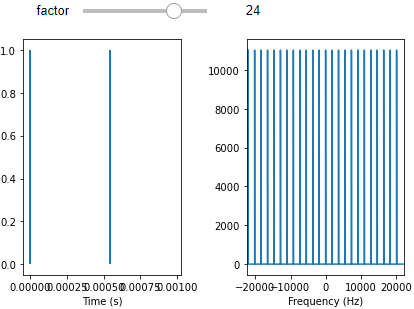
\includegraphics[width=0.7\linewidth]{resources/Images/task1_examples_1}
        \caption{Изучение примеров (влияние коэффициента выборки).}
        \label{fig:task1_examples_1}
    \end{figure}

    \begin{figure}[H]
        \centering
        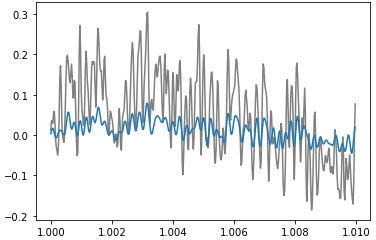
\includegraphics[width=0.7\linewidth]{resources/Images/task1_examples_2}
        \caption{Изучение примеров (cравнение исходного и дискретизированного сигналов).}
        \label{fig:task1_examples_2}
    \end{figure}

    \begin{figure}[H]
        \centering
        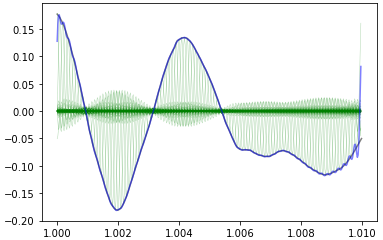
\includegraphics[width=0.7\linewidth]{resources/Images/task1_examples_3}
        \caption{Изучение примеров (сравнение исходной функции, суммы функции sinc и её сдвинутых масштабированных копий).}
        \label{fig:task1_examples_3}
    \end{figure}

    В данном упражнении были изучены все примеры в файле \texttt{chap11.ipynb}. Были изучены свертка с импульсами,
    амплитудная модуляция, сэмплинг и интерполяция \texttt{Sinc}.

    \newpage
% ---------------------------------------------- Упражнение 11.2 ----------------------------------------------
    \section{Упражнение 11.2}
    \label{sec:task2}

    В этом упражнении необходимо изучить \href{https://www.youtube.com/watch?v=cIQ9IXSUzuM}{этот} видеоролик,
    демонстрирующий теорему о выборках в действии. Кроме того, в этом видео представлена также другая полезная информация
    о выборках.

    Данный видеоролик был изучен. Была получена информация о том, что визуализировать цифровой сигнал как "ступеньки"
    не совсем верно. Также была получена информация, объясняющая, почему аналоговый сигнал в пределах человеческого
    слуха (от 20 Гц до 20 кГц) может воспроизводиться с идеальной точностью с использованием 16-битного цифрового сигнала
    44,1 кГц.


    \newpage
% ---------------------------------------------- Упражнение 11.3 ----------------------------------------------
    \section{Упражнение 11.3}
    \label{sec:task3}

    При взятии выборок из сигнала при слишком низком \texttt{framerate} большие частоты заворота дадут биения.
    И в таком случае эти компоненты будет невозможно отфильтровать, поскольку они будут неотличимы от более низких частот.
    Вариант решения - отфильтровать эти частоты до выборки с помощью фильтра низких частот (фильтр сглаживания)

    В этом упражнении необходимо применить фильтр низких частот (НЧ) к записи "Соло на барабане" до выборки. Затем опять
    с помощью фильтра НЧ удалить спектральные копии, вызванные выборкой.

    Итак, считаем файл.

    \begin{lstlisting}[caption= Чтение файла., label={lst:task3_wave}]
swave = read_wave('resources/Sounds/task3_kevcio_amen_break_a_160_bpm.wav')
wave.normalize()
wave.plot()
wave.make_audio()   \end{lstlisting}

    \begin{figure}[h]
        \centering
        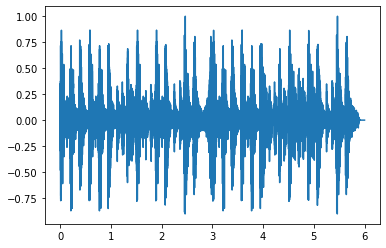
\includegraphics[width=0.8\linewidth]{resources/Images/task3_wave}
        \caption{Сигнал барабанного соло.}
        \label{fig:task3_wave}
    \end{figure}

    Теперь получим его спектр.

    \begin{lstlisting}[caption= Получение спектра., label={lst:task3_spectrum}]
spectrum = wave.make_spectrum(full=True)
spectrum.plot()     \end{lstlisting}

    \begin{figure}[H]
        \centering
        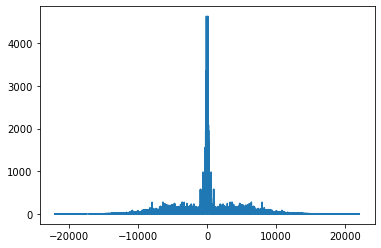
\includegraphics[width=0.8\linewidth]{resources/Images/task3_spectrum}
        \caption{Спектр нашего сигнала.}
        \label{fig:task3_spectrum}
    \end{figure}

    Уменьшим частоту дискретизации (которая сейчас равно 44,1 кГц) в 3 раза.

    \begin{lstlisting}[caption= Уменьшение частоты дискретизации., label={lst:task3_spectrum}]
factor = 3
framerate = wave.framerate / factor
cutoff = framerate / 2 - 1      \end{lstlisting}

    Применим фильтр сглаживания (фильтр НЧ), чтобы удалить частоты выше новой частоты свертки (\texttt{framerate/2}).

    \begin{lstlisting}[caption= Применение фильтра НЧ., label={lst:task3_low_pass_spectrum}]
spectrum.low_pass(cutoff)
spectrum.plot()
filtered = spectrum.make_wave()
filtered.make_audio()       \end{lstlisting}

    Полученный сигнал стал более глухим, однако это неплохой результат.

    Теперь используем функцию \texttt{sample}, описанную в файле \texttt{chap11.ipynb}.

    \begin{lstlisting}[caption= Дискретизация сигнала., label={lst:task3_spectrum_sampled}]
sampled = sample(filtered, factor)
sampled.make_audio()
sampled_spectrum = sampled.make_spectrum(full=True)
sampled_spectrum.plot()     \end{lstlisting}

    \begin{figure}[H]
        \centering
        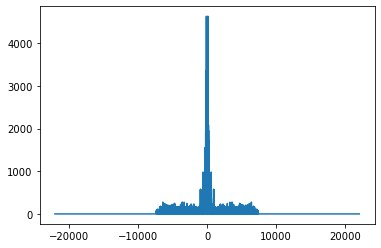
\includegraphics[width=0.82\linewidth]{resources/Images/task3_low_pass_spectrum}
        \caption{Спектр сигнала с отфильтрованными нижними частотами.}
        \label{fig:task3_low_pass_spectrum}
    \end{figure}

    \begin{figure}[H]
        \centering
        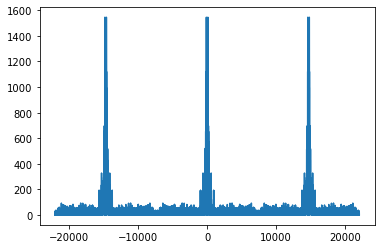
\includegraphics[width=0.82\linewidth]{resources/Images/task3_spectrum_sampled}
        \caption{Спектр сэмплированного сигнала.}
        \label{fig:task3_spectrum_sampled}
    \end{figure}

    Результат содержит копии спектра около 20 кГц. Их очень хорошо видно на спектре (Рис.\ref{fig:task3_spectrum_sampled}).
    При прослушивании очень заметны новые звонкие звуки.

    Избавимся от спектральных копий, повторно применим фильтр НЧ.


    \begin{lstlisting}[caption= Повторное применение фильтра НЧ., label={lst:task3_spectrum_sampled_low_pass}]
sampled_spectrum.low_pass(cutoff)
sampled_spectrum.plot()     \end{lstlisting}

    \begin{figure}[h]
        \centering
        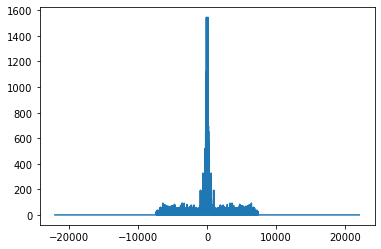
\includegraphics[width=0.7\linewidth]{resources/Images/task3_spectrum_sampled_low_pass}
        \caption{Спектр сэмплированного сигнала после применения фильтра НЧ.}
        \label{fig:task3_spectrum_sampled_low_pass}
    \end{figure}

    Масштабируем полученный спектр и сравним его со спектром до дискретизации.

    \begin{lstlisting}[caption= Сравнение спектров., label={lst:task3_compare_spectrum}]
sampled_spectrum.scale(factor)
spectrum.plot()
sampled_spectrum.plot()
spectrum.max_diff(sampled_spectrum)     \end{lstlisting}

    \begin{figure}[H]
        \centering
        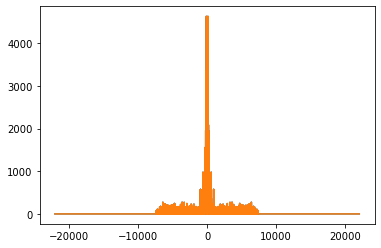
\includegraphics[width=0.7\linewidth]{resources/Images/task3_compare_spectrum}
        \caption{Сравнение спектров до и после дискретизации.}
        \label{fig:task3_compare_spectrum}
    \end{figure}

    Как мы видим из Рис\ref{fig:task3_compare_spectrum}, разница между спектрами до и после дискретизации небольшая
    (максимальная разница составляет \texttt{1.8189894035458565e-12}).

    Теперь преобразуем спектр обратно в \texttt{wave} и сравним полученный результат с оригинальным texttt{wave}.

    \begin{lstlisting}[caption= Сравнение \texttt{wave}., label={lst:task3_compare_wave}]
interpolated = sampled_spectrum.make_wave()
filtered.plot()
interpolated.plot()
interpolated.make_audio()
    \end{lstlisting}

    \begin{figure}[h]
        \centering
        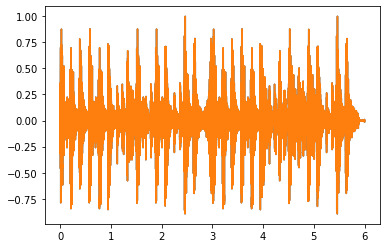
\includegraphics[width=0.8\linewidth]{resources/Images/task3_compare_wave}
        \caption{Сравнение интерполированной и фильтрованной \texttt{wave}.}
        \label{fig:task3_compare_wave}
    \end{figure}

    Как мы видим, разница между интерполированным и фильтрованным сигналом минимальна.
    Если быть точнее, максимальная разница составляет \texttt{5.56290642113787e-16}. Звук тоже не отличается.


    В данном упражнении на сигнал был применён фильтр НЧ до выборки, а после неё с его же помощью были удалены
    спектральные копии, вызванные выборкой. Таким образом нам удалось интерполировать сигнал с наименьшими потерями
    для звука.

    \newpage

% ---------------------------------------------- Выводы ----------------------------------------------
    \section{Выводы}
    \label{sec:conclusions}

    В ходе выполнения данной лабораторной работы были изучены модуляция и выборка.
    Также были изучены примеры в файле в файле \texttt{chap11.ipynb} и просмотрен полезный видеоролик.

    Кроме того, был применён способ, использующий фильтр НЧ, для интерполирования сигнала. Полученный сигнал
    минимально отличается от того, который был до интерполяции.

\end{document}